\documentclass{article}

\usepackage{tikz}
\usetikzlibrary{decorations.pathmorphing}
\usetikzlibrary{patterns}
\usetikzlibrary{arrows.meta}

\begin{document}
    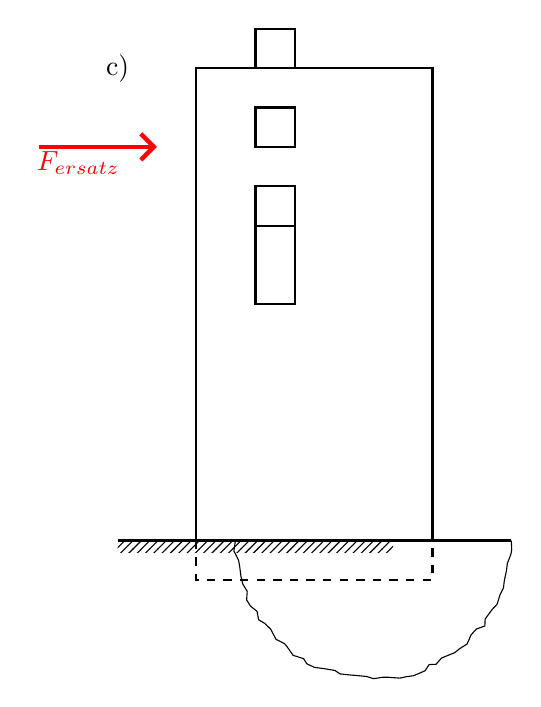
\begin{tikzpicture}[pencildraw/.style={
        black,
        decorate,
        decoration={random steps,segment length=3pt,amplitude=1pt}
        }]

    %Building
    \draw[black, thick] (0, -4) rectangle (3, 2);
    \draw[black, thick] (0.75, 2) rectangle (1.25, 2.5);
    \draw[black, thick] (0.75, 1) rectangle (1.25, 1.5);
    \draw[black, thick] (0.75, 0) rectangle (1.25, 0.5);
    \draw[black, thick] (0.75, -1) rectangle (1.25, 0.5);
    \draw[black, thick, dashed] (0, -4) -- (0, -4.5) -- (3, -4.5) -- (3, -4);

    %Text
    \draw[-{Straight Barb}, red, ultra thick] (-2,1) -- (-0.5, 1);
    \node[font = \bfseries, text = red, align = left] at (-1.5, 0.8) {$F_{ersatz}$};
    \node at (-1,2) {c)};
        
    %Ground
    \draw[black, thick] (-1, -4) -- (4, -4);
    \draw[pencildraw] (4, -4) arc (0:-180:1.75);
    \draw[pattern = north east lines, draw = none] (-1, -4.15) rectangle (2.5, -4);

    \end{tikzpicture}
\end{document}